% auto-generated by build_deck_ej230.py -- do not edit by hand
% All numerical values sourced from deck_values.json
\documentclass[aspectratio=169,10pt]{beamer}

\usetheme{default}
\usepackage[utf8]{inputenc}
\usepackage[T1]{fontenc}
\usepackage{booktabs}
\usepackage{graphicx}
\usepackage{amsmath}
\usepackage{xcolor}
\usepackage{siunitx}

\definecolor{shipblue}{RGB}{20,74,130}
\definecolor{warnorange}{RGB}{210,105,30}
\definecolor{okgreen}{RGB}{0,128,0}
\setbeamercolor{structure}{fg=shipblue}
\setbeamercolor{alerted text}{fg=warnorange}
\setbeamertemplate{navigation symbols}{}
\setbeamertemplate{footline}[frame number]

% ---- macros sourced from deck_values.json -----------------------------------
\newcommand{\BarLen}{1400}
\newcommand{\NEv}{2,000}
\newcommand{\NPos}{31}
% Material properties (EJ-230 / OPSC-106, Materials.cc)
\newcommand{\LamBulk}{120}
\newcommand{\ScintYield}{9,700\,$\gamma$/MeV}
\newcommand{\PeakEm}{391}
\newcommand{\RefrIdx}{1.58}
\newcommand{\DensityGcc}{1.023}
\newcommand{\TauRise}{0.5\,ns}
\newcommand{\TauDecay}{1.5\,ns}
% Optical group velocity
\newcommand{\VGroup}{189.7\,mm/ns}
% Mylar
\newcommand{\MylarR}{0.90}
\newcommand{\MylarLoss}{0.10}
\newcommand{\MylarSL}{1.0}
\newcommand{\MylarSA}{0.1}
% SiPM
\newcommand{\PDEpeak}{62\%}
\newcommand{\SiPMModel}{AFBR-S4N66P014M}
\newcommand{\SiPMModelPDE}{AFBR-S4N66P024M}
% Attenuation -- M1 (single-exp)
\newcommand{\LamSingleL}{\ensuremath{29.2\pm1.6}\,cm}
\newcommand{\LamSingleR}{\ensuremath{29.4\pm1.6}\,cm}
\newcommand{\ChiSingleL}{2367}
\newcommand{\NzeroSingleL}{782}
% Attenuation -- M3 (exp + finite-range offset)
\newcommand{\LamPromptL}{\ensuremath{20.0\pm1.0}\,cm}
\newcommand{\COffsetL}{\ensuremath{13.3\pm1.6}\,PE}
\newcommand{\ChiExpoffL}{1070}
% Attenuation -- M2 (constrained double-exp)
\newcommand{\LamShortL}{\ensuremath{9.0\pm0.4}\,cm}
\newcommand{\LamLongL}{\ensuremath{38.9\pm0.8}\,cm}
\newcommand{\AmpShortL}{\ensuremath{2104}}
\newcommand{\AmpLongL}{\ensuremath{373}}
\newcommand{\ChiMtwo}{101}
% Attenuation -- M4 (tail slope)
\newcommand{\LamTailL}{\ensuremath{38.1\pm0.8}\,cm}
\newcommand{\LamTailR}{\ensuremath{38.1\pm0.8}\,cm}
\newcommand{\ChiTailL}{87.8}
\newcommand{\DTail}{40}
% NPE at key positions
\newcommand{\ActualNearL}{2675}
\newcommand{\NpeLeftZero}{60.1}         % x=0 exact (center_point_npe)
\newcommand{\NpeRightZero}{59.9}
\newcommand{\NpeCentralLeft}{62.0}  % |x|<=100 mm average
\newcommand{\NpeCentralRight}{61.9}
% Near / far ends
\newcommand{\NpeNearLeft}{2675}
\newcommand{\NpeFarRightAtLeft}{11.4}
\newcommand{\NpeNearRight}{2667}
\newcommand{\NpeFarLeftAtRight}{11.6}
% EndTop
\newcommand{\EndtopR}{0.98}
\newcommand{\LamTailET}{\ensuremath{37.9\pm0.6}\,cm}
\newcommand{\NPECentralMylar}{62.0}   % |x|<=100 mm avg
\newcommand{\NPECentralET}{155.1}
\newcommand{\NPEPointMylar}{60.1}        % x=0 exact
\newcommand{\NPEPointET}{151.0}
% sigma_eq = sigma(tL-tR)/sqrt(2)
\newcommand{\SigEqAtMsixnine}{\ensuremath{485\pm38}\,ps}
\newcommand{\SigEqAtMfour}{\ensuremath{249\pm17}\,ps}
\newcommand{\SigEqAtZero}{\ensuremath{140\pm4}\,ps}
\newcommand{\SigEqAtFour}{\ensuremath{244\pm13}\,ps}
\newcommand{\SigEqAtSixnine}{\ensuremath{434\pm31}\,ps}
% Apparent estimator velocities (not photon propagation speed)
\newcommand{\VappFPT}{263.6\,mm/ns}
\newcommand{\VappSUMfour}{210.3\,mm/ns}
\newcommand{\VappTfifty}{275.5\,mm/ns}
% Photon budget fractions
\newcommand{\PctSurfaceBulk}{89.8}
\newcommand{\PctEsc}{4.63}
\newcommand{\PctSiPM}{5.54}
\newcommand{\PctDet}{3.41}
\newcommand{\PDEeff}{0.62}
% Bootstrap summary (C++/OpenMP, 200 replicas) -- M4 tail
\newcommand{\BootTailMed}{38.2}
\newcommand{\BootTailPlo}{37.2}
\newcommand{\BootTailPhi}{39.2}
\newcommand{\BootNReplicas}{200}

\title[End-only + Mylar EJ-230]{%
  End-only + Mylar-wrapped EJ-230 bar:\\
  Optical simulation study}
\subtitle{Geant4 11.4.0 / SSLG4-OPSim}
\author{R.\ R\'ios (ULS)}
\institute{SHiP Collaboration Meeting}
\date{2026-06-14}

\begin{document}

% ---- FRAME 1: Title ----------------------------------------------------------
\begin{frame}
  \titlepage
\end{frame}

% ---- FRAME 2: Motivation & scope --------------------------------------------
\begin{frame}{Motivation \& scope}
  \begin{columns}[T]
    \column{0.55\textwidth}
    \begin{itemize}
      \item \textbf{Controlled optical study:} readout \emph{only} at the
            two ends ($\pm X$ faces); all other faces wrapped in Mylar.
            Not a final detector configuration.
      \item \textbf{Goals:}
        \begin{itemize}
          \item Isolate end-readout optical response.
          \item Characterize multi-component attenuation with Mylar.
          \item Benchmark timing estimators in a clean geometry.
        \end{itemize}
      \item \NPos\ beam positions ($x=-690\ldots+690$\,mm),
            \NEv\ $\mu^-$ events per position.
    \end{itemize}
    \column{0.43\textwidth}
    \begin{block}{This study}
      \textbf{End-only + Mylar} = extreme limit.
      Photons either exit to an end SiPM,
      \textbf{escape} through the bar boundaries,
      or are absorbed (surface or bulk) after multiple reflections.
    \end{block}
    \begin{alertblock}{\small No TB counterpart}
      \small This configuration has \alert{no direct test-beam counterpart}
      (April-2026 TB used top readout + Tyvek).
    \end{alertblock}
    \begin{alertblock}{\small Electronic jitter not included}
      \small SPTR ($\approx106$\,ps) and FastIC ($\approx10$\,ps) are
      post-processing steps, not folded into $\sigma_{\rm eq}$ shown here.
    \end{alertblock}
  \end{columns}
\end{frame}

% ---- FRAME 3: Geometry & simulation setup ------------------------------------
\begin{frame}{Geometry \& simulation setup}
  \begin{columns}[T]
    \column{0.55\textwidth}
    \begin{itemize}
      \item \textbf{Bar:} EJ-230 (OPSC-106),
            $\BarLen \times 60 \times 10$\,mm$^3$; long axis $X$.
      \item \textbf{End-left SiPMs} (IDs 0--7): $-X$ face.
            \textbf{End-right SiPMs} (IDs 8--15): $+X$ face.
      \item \textbf{Wrapping:} Mylar dielectric surface on $\pm Y,\pm Z$.
            $R=\MylarR$, specular lobe $=\MylarSL$,
            $\sigma_\alpha=\MylarSA^\circ$.
      \item \textbf{SUM4:} leading-edge at 4\,PE;
            groups $\{0\text{--}3\}/\{4\text{--}7\}$ (left),
            $\{8\text{--}11\}/\{12\text{--}15\}$ (right).
      \item \textbf{Rayleigh scattering:} active
            ($\lambda_{\rm Rayl}\approx150$\,cm at peak;
            $\propto\lambda^4$; Materials.cc:45--55).
    \end{itemize}
    \column{0.43\textwidth}
    \begin{block}{Key parameters}
      \small
      \begin{tabular}{ll}
        \toprule
        Scint.~yield    & \ScintYield \\
        Emission peak   & \PeakEm\,nm \\
        Bulk $\lambda$ (ABSLENGTH) & \LamBulk\,cm \\
        $n$ (flat)      & \RefrIdx \\
        $v_g = c/n$     & \VGroup \\
        $\tau_r/\tau_d$ & \TauRise/\TauDecay \\
        Mylar $R$       & \MylarR \\
        \bottomrule
      \end{tabular}
    \end{block}
    \begin{alertblock}{\small Note on $v_g$}
      \small No \texttt{GROUPVEL} property set.
      Geant4 computes $v_g=c/n=\VGroup$ from flat $n=\RefrIdx$.
    \end{alertblock}
  \end{columns}
\end{frame}

% ---- FRAME 4: Photon yield vs position ---------------------------------------
\begin{frame}{Photon yield at ends vs.\ beam position}
  \begin{columns}[T]
    \column{0.65\textwidth}
    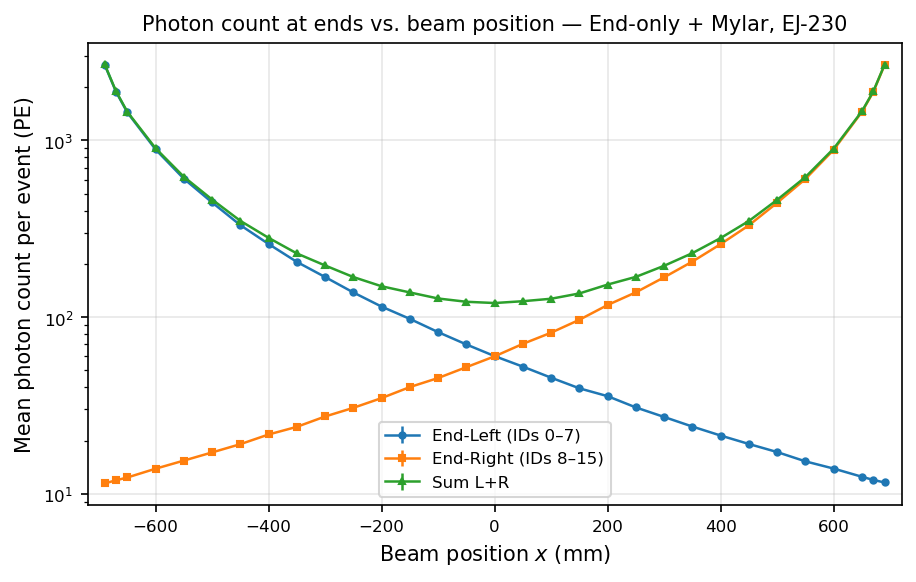
\includegraphics[width=\textwidth]{figures/fig_npe_vs_x.png}
    \column{0.33\textwidth}
    \begin{block}{Representative values}
      \small
      Near \textbf{left} end ($x=-690$\,mm):\\
      \quad End-Left (near) $\approx \NpeNearLeft$\,PE\\
      \quad End-Right (far) $\approx \NpeFarRightAtLeft$\,PE
      \medskip

      \textbf{Center} ($x=0$, center-point):\\
      \quad End-Left $\approx \NpeLeftZero$\,PE\\
      \quad Central avg ($|x|\!\leq\!100$\,mm): $\approx\NpeCentralLeft$\,PE

      \medskip
      Near \textbf{right} end ($x=+690$\,mm):\\
      \quad End-Right (near) $\approx \NpeNearRight$\,PE\\
      \quad End-Left (far) $\approx \NpeFarLeftAtRight$\,PE
    \end{block}
    \begin{alertblock}{\small Two-scale structure}
      \small Near-end: prompt contribution.
      Center: $\approx\NpeCentralLeft$\,PE residual sustained by
      Mylar recirculation (many bounces at $R=\MylarR$).
    \end{alertblock}
  \end{columns}
\end{frame}

% ---- FRAME 5: Bulk vs system response ----------------------------------------
\begin{frame}{Bulk attenuation and longitudinal light-yield scales}
  \begin{columns}[T]
    \column{0.50\textwidth}
    \begin{block}{ABSLENGTH = \LamBulk\,cm (material property)}
      \small
      Describes absorption along the \textbf{actual optical path length} $s$:
      $P_{\rm bulk}(s)=e^{-s/\lambda_{\rm bulk}}$.
      A photon propagating 70\,cm longitudinally may traverse
      significantly more path via reflections.
      ABSLENGTH knows nothing about bar geometry or reflectors.
    \end{block}
    \begin{exampleblock}{Fitted longitudinal scale (system observable)}
      \small
      NPE vs.\ distance $d$ combines: bulk absorption (over actual $s$),
      Rayleigh scattering, geometry, repeated Mylar surface losses,
      SiPM acceptance, and PDE.
      \textbf{Any fitted scale is a system-dependent empirical parameter.}
    \end{exampleblock}
    \column{0.48\textwidth}
    \begin{alertblock}{Why single-exp fails}
      \small
      Three numbers inconsistent with $N_0\,e^{-d/\lambda}$:
      \begin{enumerate}
        \item Two-point: $\lambda\approx19$\,cm
        \item Fit: $N_0=\NzeroSingleL$\,PE, $\lambda=\LamSingleL$
        \item Observed at $d\approx0$: $\ActualNearL$\,PE
      \end{enumerate}
      Items (2) and (3) disagree by $\approx3.6\times$.\\
      $\chi^2/\mathrm{ndf}=\ChiSingleL$: catastrophic.
      \medskip
      \textbf{Cause:} superposition of a prompt component
      and a long-range contribution with finite-range offset.
    \end{alertblock}
  \end{columns}
\end{frame}

% ---- FRAME 6: Attenuation curve ----------------------------------------------
\begin{frame}{Attenuation: four models and empirical tail slope}
  \begin{columns}[T]
    \column{0.65\textwidth}
    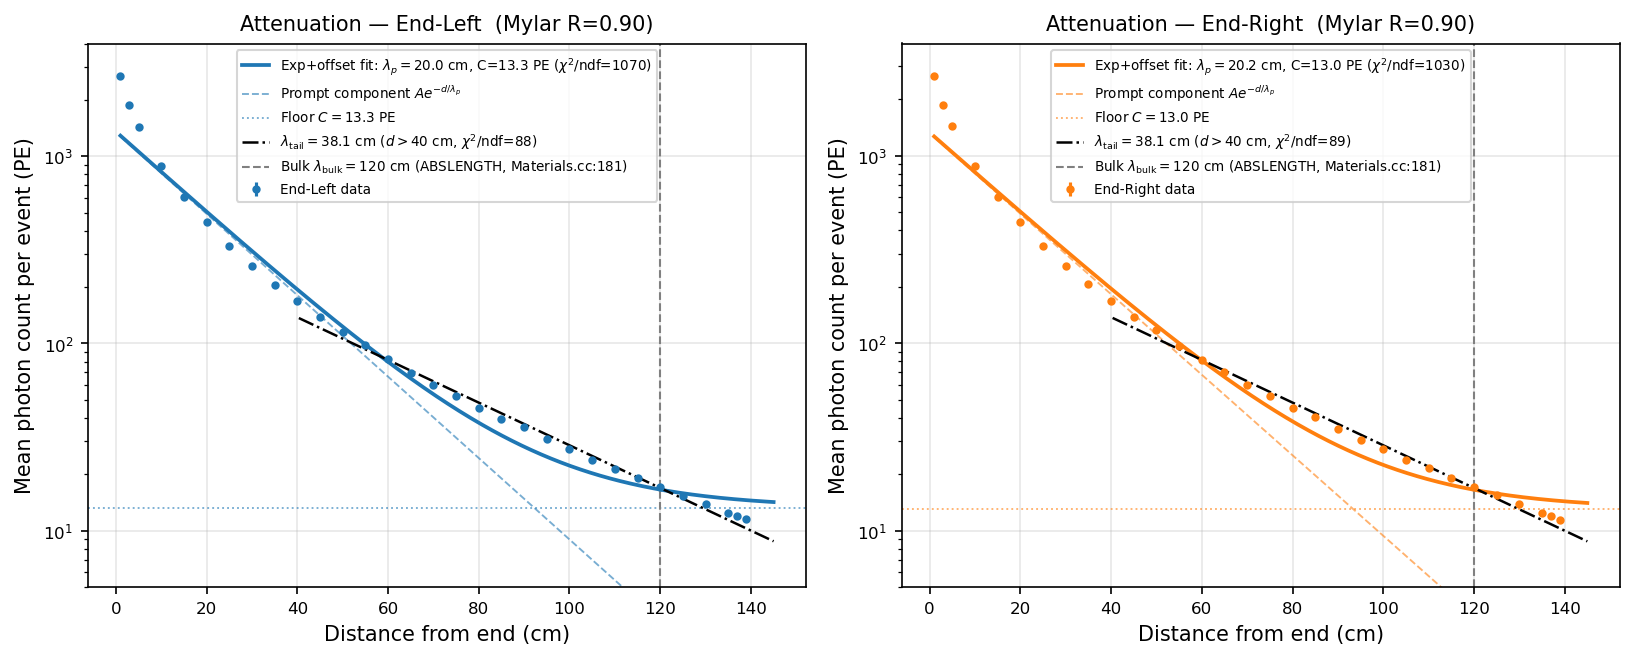
\includegraphics[width=\textwidth]{figures/fig_attenuation.png}
    \column{0.33\textwidth}
    \begin{block}{M3 result (exp + finite-range offset)}
      \small
      $N(d) = A\,e^{-d/\lambda_p} + C$
      \medskip

      $\lambda_p = \LamPromptL$ (prompt scale)\\
      $C = \COffsetL$ (finite-range offset)\\
      $\chi^2/\mathrm{ndf} = \ChiExpoffL$
    \end{block}
    \begin{block}{M4 (empirical tail slope)}
      \small
      $d>\DTail$\,cm:\quad $\lambda_{\rm tail}=\LamTailL$\\
      $\chi^2/\mathrm{ndf}=\ChiTailL$
    \end{block}
    \begin{alertblock}{\small All $\chi^2/\mathrm{ndf}\gg1$}
      \small All models are \emph{empirical approximations}.
      $\lambda_p$, $\lambda_{\rm tail}$ are system-dependent scales,
      not the EJ-230 bulk ABSLENGTH (\LamBulk\,cm).
    \end{alertblock}
  \end{columns}
\end{frame}

% ---- FRAME 7: Model comparison -----------------------------------------------
\begin{frame}{Model comparison: M1, M2, M3, M4 (left side)}
  \begin{columns}[T]
    \column{0.65\textwidth}
    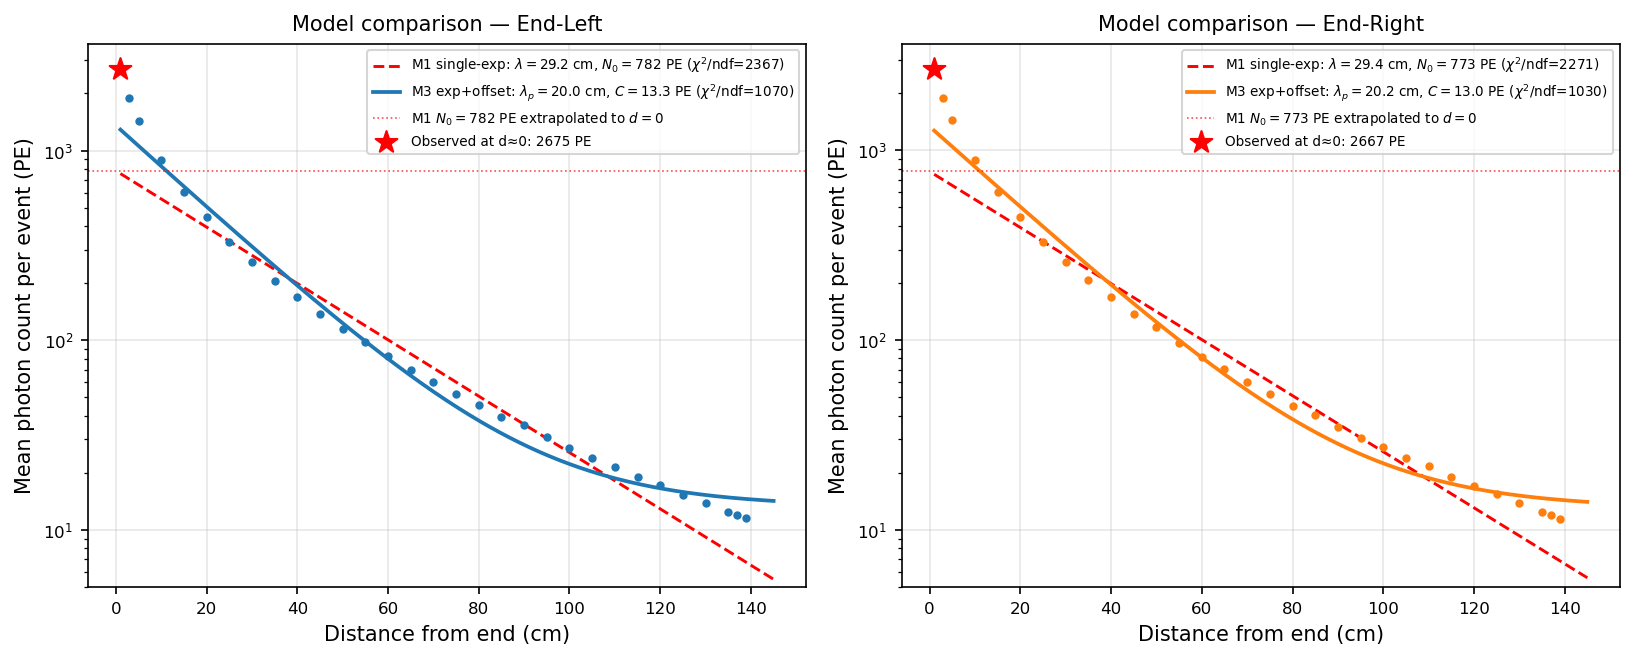
\includegraphics[width=\textwidth,height=0.80\textheight,keepaspectratio]{figures/fig_attenuation_twocomp.png}
    \column{0.33\textwidth}
    \begin{block}{Fit diagnostics (covariance errors)}
      \tiny
      \begin{tabular}{lrr}
        \toprule
        Parameter & Value & $\chi^2/\mathrm{ndf}$ \\
        \midrule
        M1: $\lambda$             & \LamSingleL  & \ChiSingleL \\
        M3: $\lambda_p$           & \LamPromptL  & \ChiExpoffL \\
        M3: $C$ (offset)          & \COffsetL    & --- \\
        M2: $A_s$                 & \AmpShortL   & \ChiMtwo \\
        M2: $\lambda_s$           & \LamShortL   & --- \\
        M2: $A_l$                 & \AmpLongL    & --- \\
        M2: $\lambda_l$           & \LamLongL    & --- \\
        M4: $\lambda_{\rm tail}$  & \LamTailL    & \ChiTailL \\
        \bottomrule
      \end{tabular}
    \end{block}
    \begin{alertblock}{\small Empirical approximations}
      \small
      Red star: observed NPE $\approx\ActualNearL$\,PE at $d\approx0$.\\
      M1 $N_0=\NzeroSingleL$\,PE: factor $\approx3.6$ off.\\
      M2 identifies two empirical scales but
      $\chi^2/\mathrm{ndf}=\ChiMtwo\gg1$:
      not an exact description.
    \end{alertblock}
  \end{columns}
\end{frame}

% ---- FRAME 8: Far-end light yield -------------------------------------------
\begin{frame}{Far-end light yield: where reflector quality matters}
  \begin{columns}[T]
    \column{0.55\textwidth}
    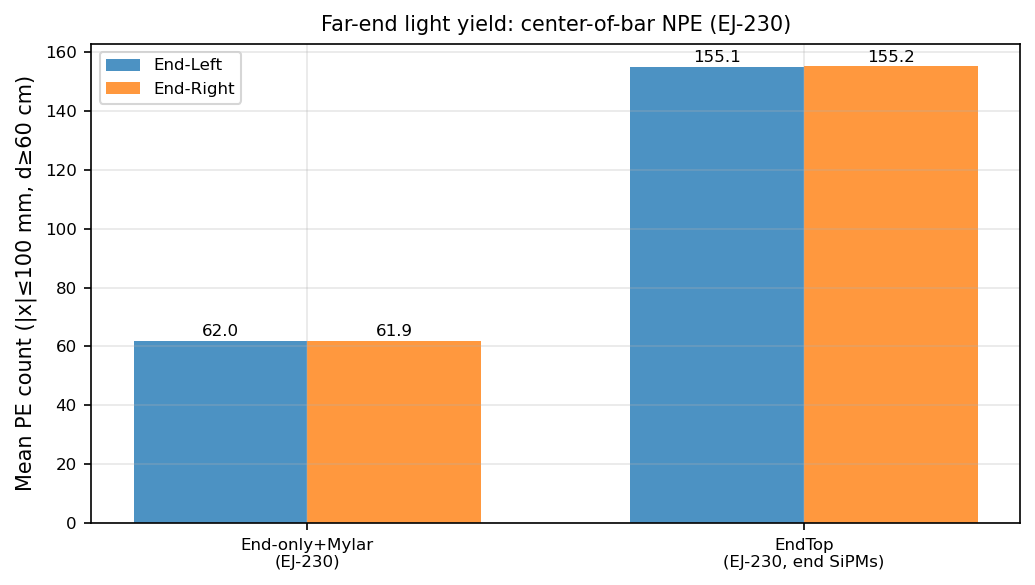
\includegraphics[width=\textwidth]{figures/fig_far_end_yield.png}
    \column{0.43\textwidth}
    \begin{block}{Central-region NPE ($|x|\leq100$\,mm)}
      \small
      \begin{tabular}{lrr}
        \toprule
        Config & $R$ & NPE \\
        \midrule
        End-only+Mylar & \MylarR & \NPECentralMylar\,PE \\
        EndTop         & \EndtopR & \NPECentralET\,PE \\
        \bottomrule
      \end{tabular}
      \medskip
      Ratio EndTop/Mylar $\approx 2.5\times$.
    \end{block}
    \begin{alertblock}{\small Interpretation}
      \small
      Both see photons after $\geq60$\,cm and many
      reflections.
      Mylar loss/interaction: $1{-}R=\MylarLoss$ (10\%).
      Accumulated over many bounces, this strongly suppresses
      far-end yield.
      \smallskip
      $2.5\times$ difference is \textbf{consistent with}
      higher-$R$ boundaries in EndTop ($R=\EndtopR$),
      but this is a \textbf{configuration-level result}.
    \end{alertblock}
  \end{columns}
\end{frame}

% ---- FRAME 9: Apples-to-apples EndTop ----------------------------------------
\begin{frame}{Apples-to-apples: End-only+Mylar vs.\ EndTop (end SiPMs only)}
  \begin{columns}[T]
    \column{0.65\textwidth}
    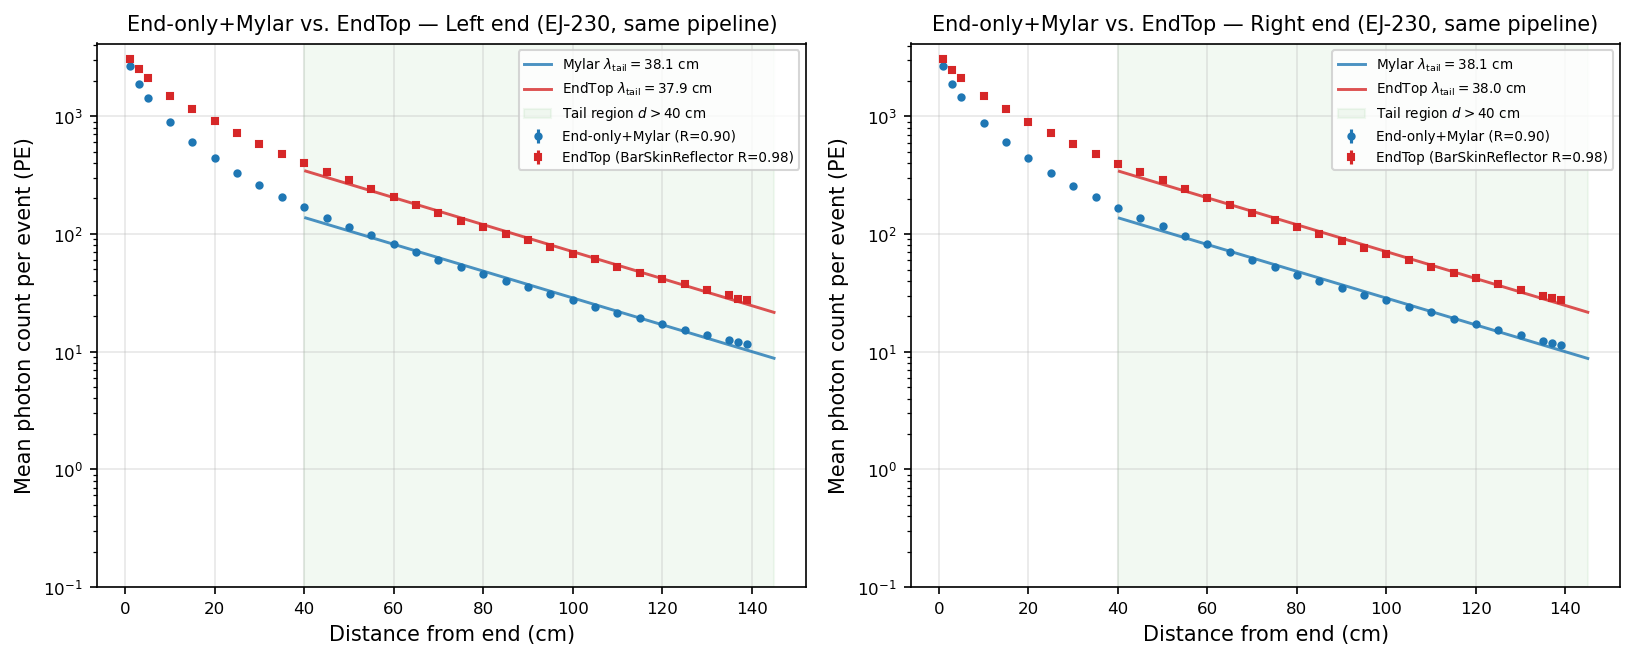
\includegraphics[width=\textwidth]{figures/fig_endtop_comparison.png}
    \column{0.33\textwidth}
    \begin{block}{Identical pipeline}
      \small
      Both datasets: same end-SiPM-only selection,
      same models, same tail-fit range $d>\DTail$\,cm.
    \end{block}
    \begin{block}{Empirical tail slope ($d>\DTail$\,cm)}
      \tiny
      \begin{tabular}{lr}
        \toprule
        Config & $\lambda_{\rm tail}$ \\
        \midrule
        End-only+Mylar & \LamTailL \\
        EndTop (end SiPMs) & \LamTailET \\
        \bottomrule
      \end{tabular}

      Numerically similar slopes in this fit range.
      Does \emph{not} establish reflector independence
      or exclude model error.
    \end{block}
    \begin{alertblock}{\small Key conclusion}
      \small
      NPE amplitude at center differs $2.5\times$.
      The tail slope is not the discriminating observable;
      the \textbf{absolute light yield} is.
      Difference is consistent with higher-$R$ boundaries
      (configuration-level).
    \end{alertblock}
  \end{columns}
\end{frame}

% ---- FRAME 10: Timing distributions -----------------------------------------
\begin{frame}{Arrival-time distributions: FPT at representative positions}
  \begin{columns}[T]
    \column{0.65\textwidth}
    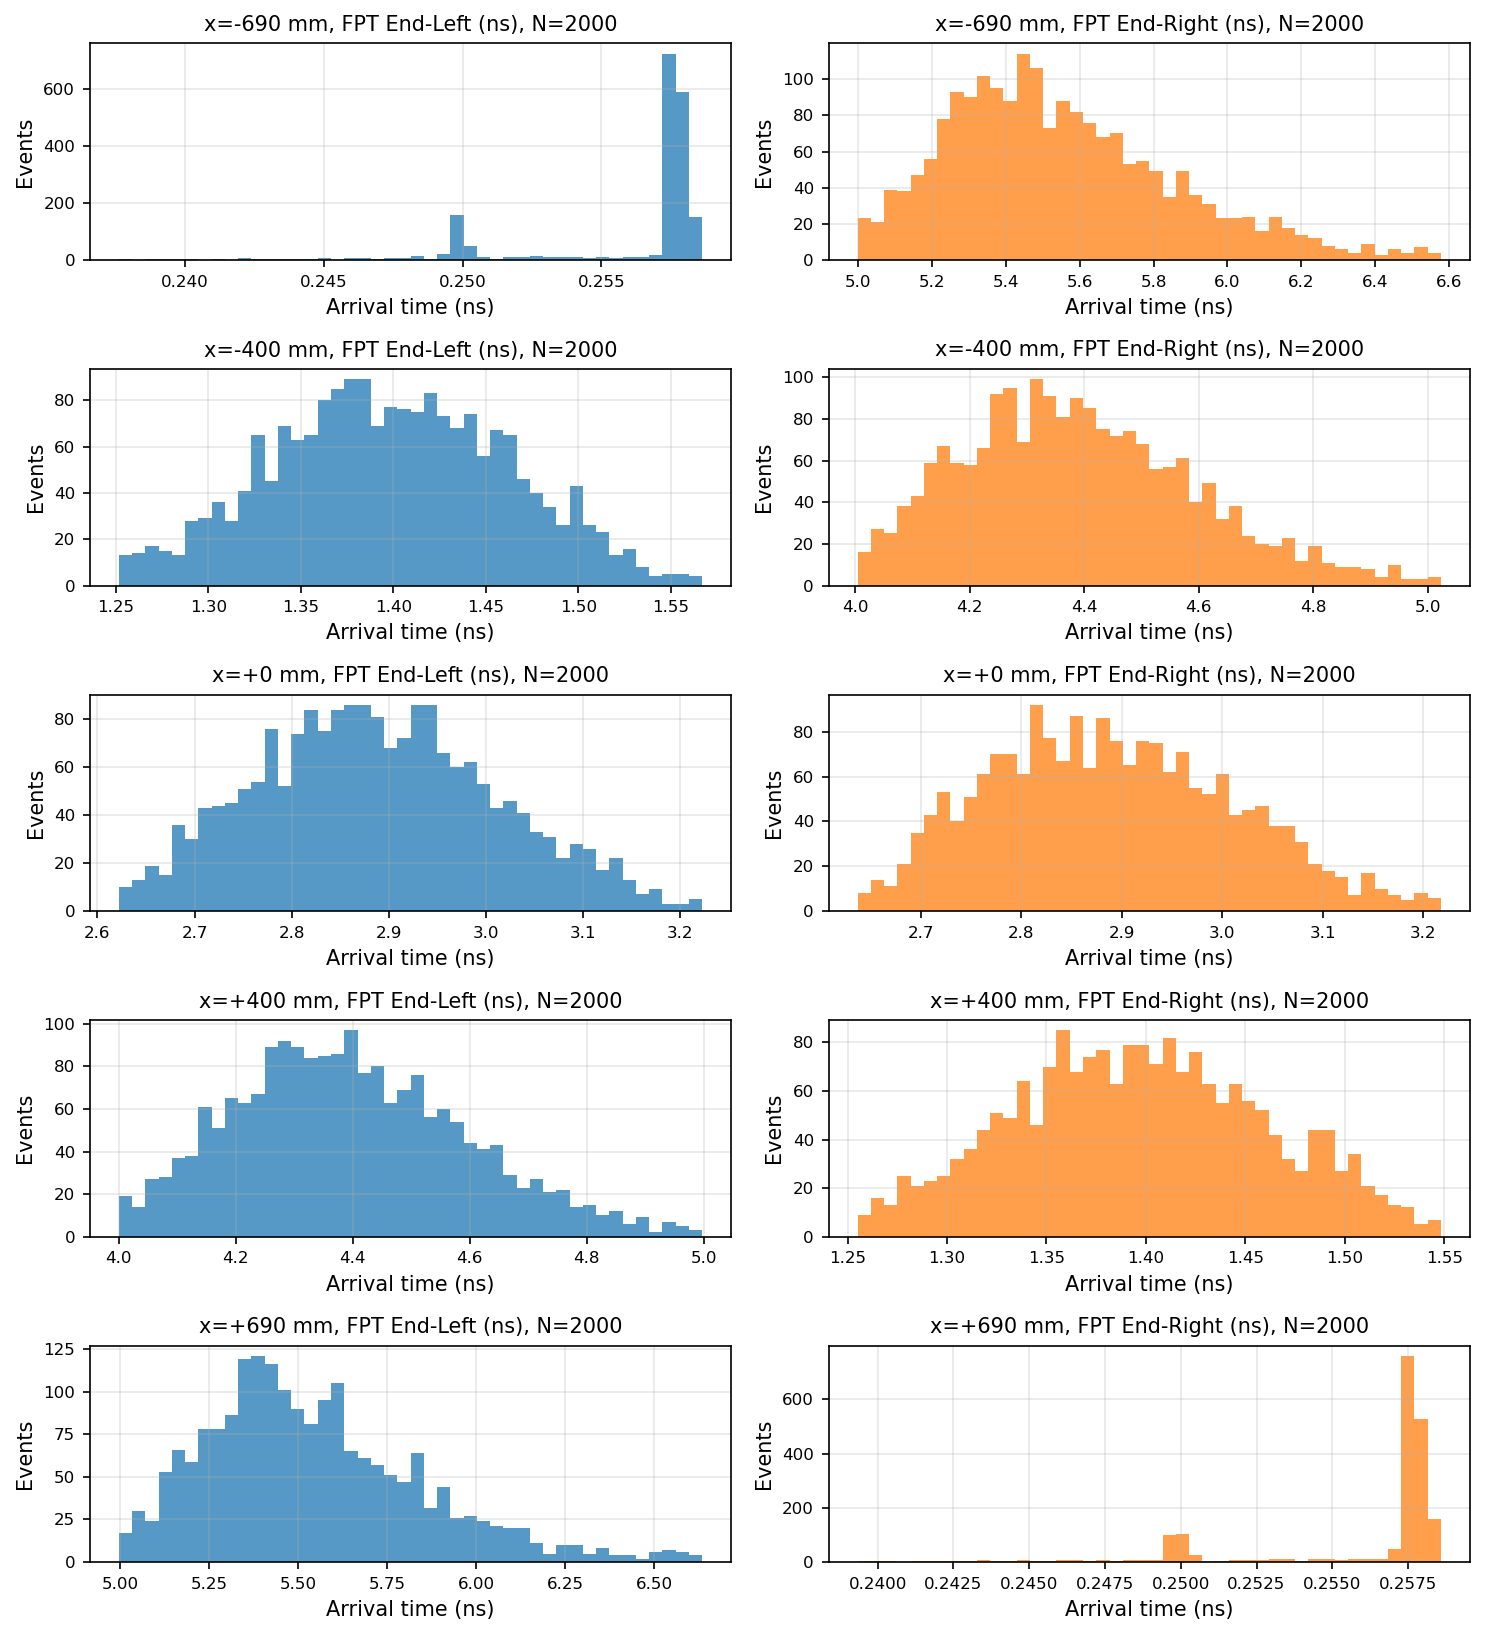
\includegraphics[width=\textwidth,height=0.78\textheight,keepaspectratio]{figures/fig_timing_histograms.png}
    \column{0.33\textwidth}
    \begin{block}{Distributions shown}
      \small
      FPT at End-Left and End-Right.\\
      $x\in\{-690,-400,0,+400,+690\}$\,mm.\\
      $N = \NEv$ events/position.
    \end{block}
    \begin{alertblock}{\small Shape}
      \small Distribution shifts later and broadens
      as beam moves from the SiPM:
      longer path, fewer photons, estimator-dependent
      response to photon-population size.
    \end{alertblock}
  \end{columns}
\end{frame}

% ---- FRAME 11: FPT vs t50 ---------------------------------------------------
\begin{frame}{FPT vs.\ $t_{50}$: estimator comparison}
  \begin{columns}[T]
    \column{0.65\textwidth}
    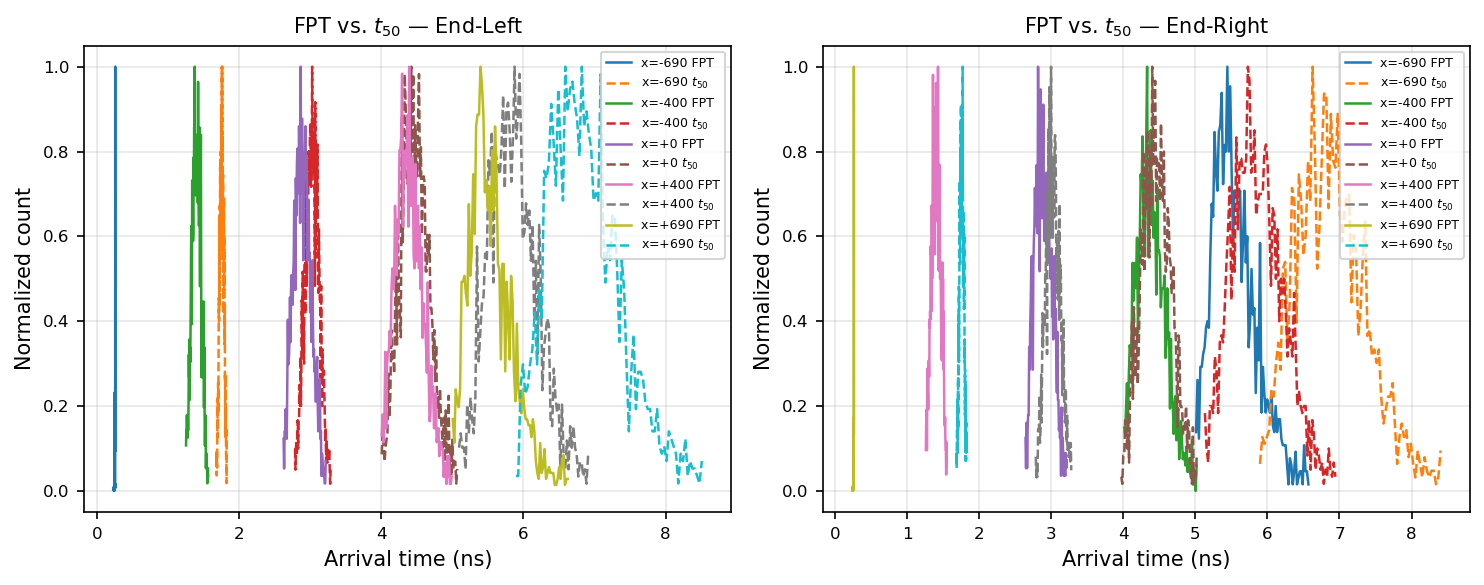
\includegraphics[width=\textwidth]{figures/fig_fpt_vs_t50.png}
    \column{0.33\textwidth}
    \begin{block}{FPT vs.\ $t_{50}$}
      \small
      FPT: minimum arrival time per event.\\
      $t_{50}$: per-event median --- less sensitive
      to photon-population size effects.
      \medskip
      $t_{50}$ is systematically later than FPT;
      offset grows with distance.
    \end{block}
    \begin{alertblock}{\small Estimator-dependent response}
      \small
      Both FPT and $t_{50}$ slopes exhibit
      position-dependent apparent velocities.
      These reflect the \textbf{estimator-dependent apparent
      longitudinal response}: systematic shifts of the
      estimator mean with photon-population size and
      reflection path-length distribution.
      This is a sampling and bias effect, not superluminal transport.
    \end{alertblock}
  \end{columns}
\end{frame}

% ---- FRAME 12: Position dependence of timing estimators ---------------------
\begin{frame}{Position dependence of timing estimators}
  \begin{columns}[T]
    \column{0.65\textwidth}
    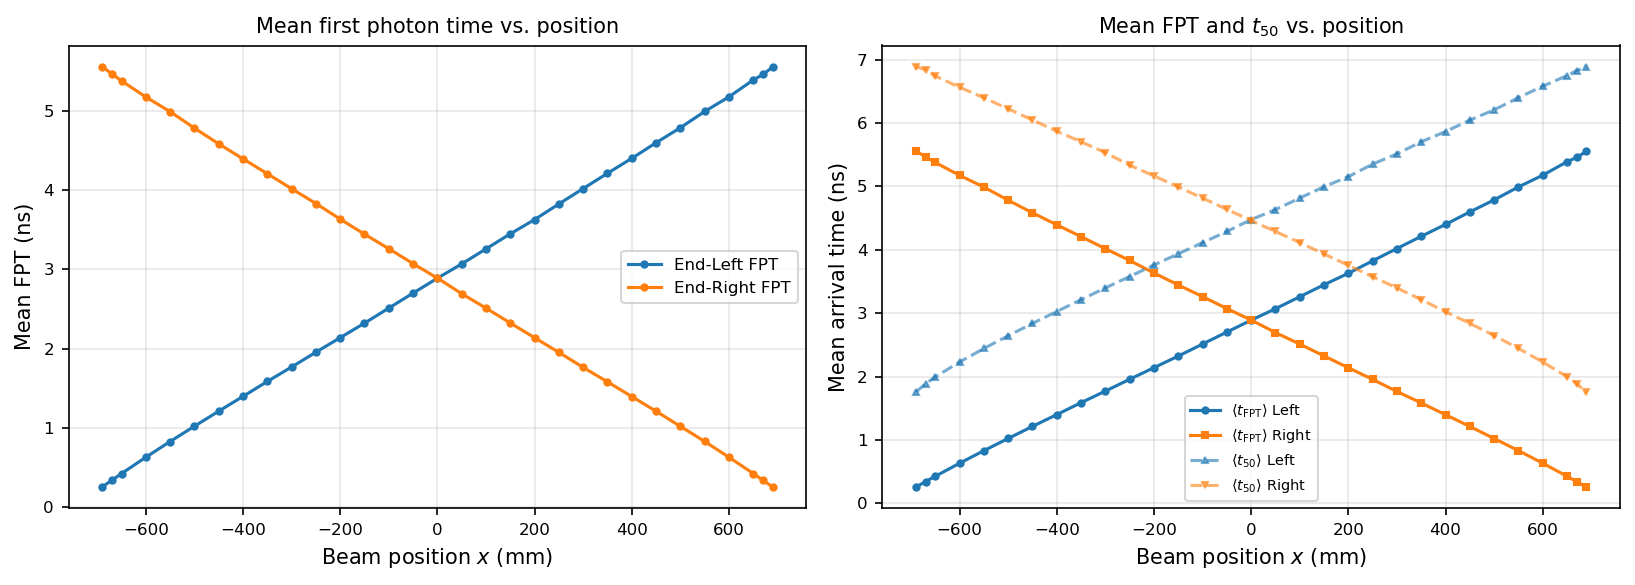
\includegraphics[width=\textwidth]{figures/fig_mean_arrival_time.png}
    \column{0.33\textwidth}
    \begin{block}{Apparent estimator velocities}
      \small
      \begin{tabular}{ll}
        \toprule
        Estimator & $v_{\rm app}$ \\
        \midrule
        SUM4 $\Delta t$  & \VappSUMfour \\
        FPT slope        & \VappFPT \\
        $t_{50}$ slope   & \VappTfifty \\
        \midrule
        $c/n$ (theory)   & \VGroup \\
        \bottomrule
      \end{tabular}
    \end{block}
    \begin{alertblock}{\small All exceed $c/n$}
      \small
      These are \textbf{estimator-dependent apparent longitudinal
      responses}, not direct measurements of photon group velocity.
      All exceed $c/n = \VGroup$\ ($n=\RefrIdx$, flat RINDEX).
      Reflects position-dependent photon-population and
      estimator biases (reflections, path-length distributions,
      threshold selection).
    \end{alertblock}
  \end{columns}
\end{frame}

% ---- FRAME 13: sigma_eq(x) --------------------------------------------------
\begin{frame}{Intrinsic timing metric $\sigma_{\rm eq}(x)$}
  \begin{columns}[T]
    \column{0.65\textwidth}
    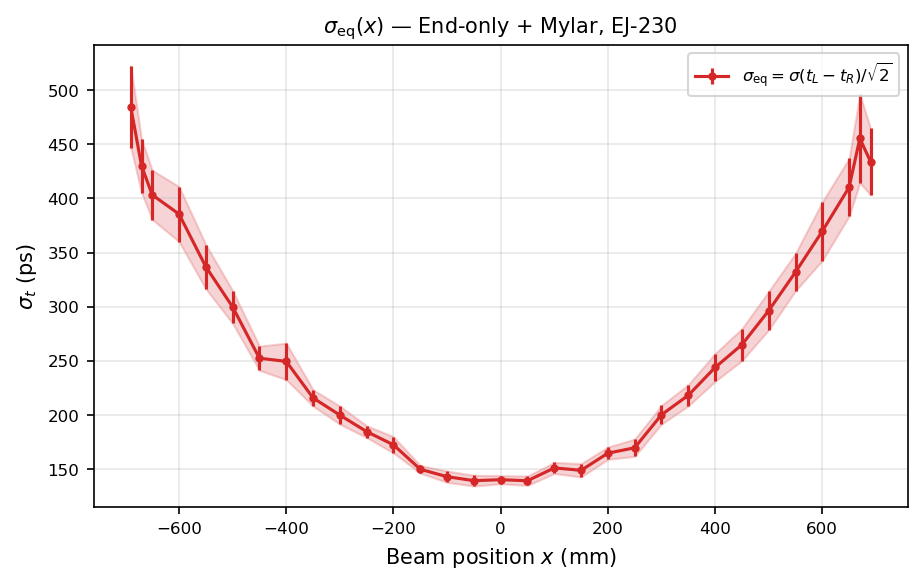
\includegraphics[width=\textwidth]{figures/fig_sigma_t.png}
    \column{0.33\textwidth}
    \begin{block}{Key values of $\sigma_{\rm eq}$}
      \small
      \begin{tabular}{ll}
        \toprule
        $x$ (mm) & $\sigma_{\rm eq}$ (ps) \\
        \midrule
        $-690$ & \SigEqAtMsixnine \\
        $-400$ & \SigEqAtMfour \\
        $0$    & \SigEqAtZero \\
        $+400$ & \SigEqAtFour \\
        $+690$ & \SigEqAtSixnine \\
        \bottomrule
      \end{tabular}
    \end{block}
    \begin{alertblock}{\small Definition and caveats}
      \small
      $\sigma_{\rm eq}\equiv\sigma(t_L-t_R)/\sqrt{2}$
      (SUM4, core Gaussian fit).
      \textbf{Equals per-end resolution only under equal,
      independent-end assumptions} --- which break down at
      the bar ends where NPE is strongly asymmetric.
      \medskip
      Intrinsic optical+estimator only.
      SPTR and electronics \alert{not} included.
    \end{alertblock}
  \end{columns}
\end{frame}

% ---- FRAME 14: Photon budget -------------------------------------------------
\begin{frame}{Photon budget --- End-only + Mylar}
  \begin{columns}[T]
    \column{0.65\textwidth}
    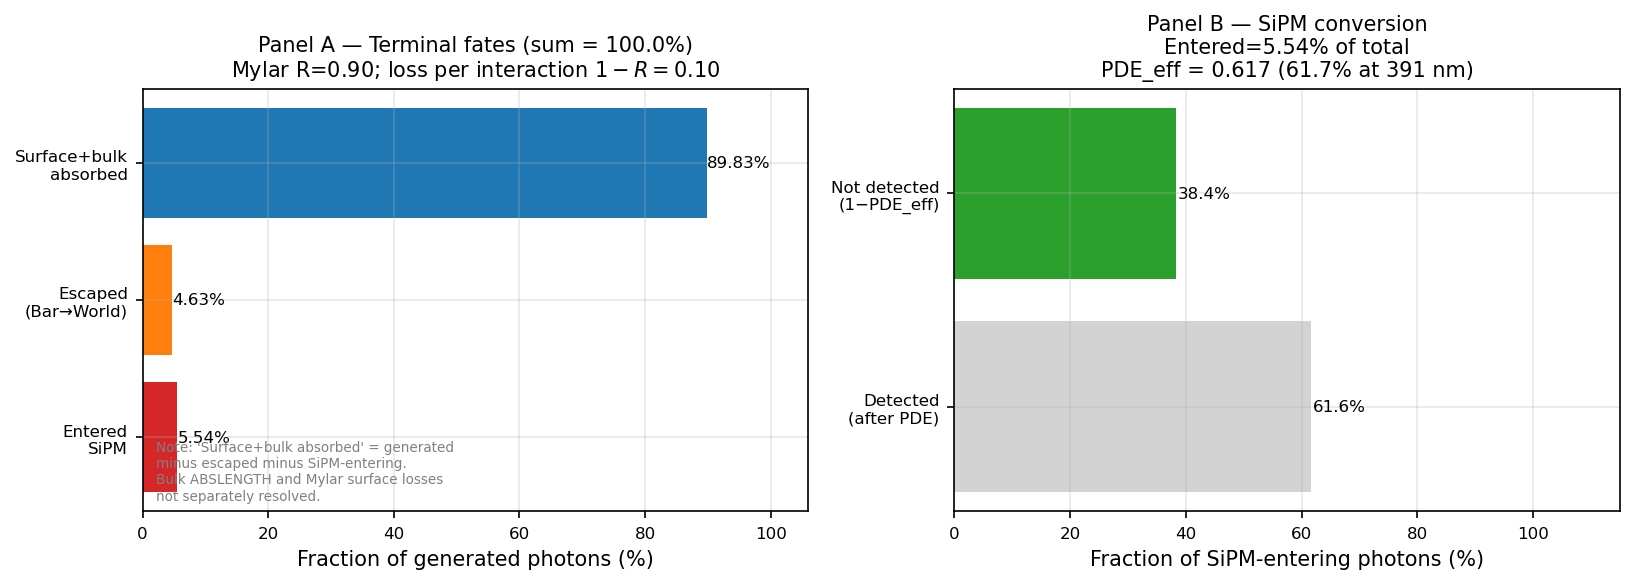
\includegraphics[width=\textwidth]{figures/fig_photon_budget.png}
    \column{0.33\textwidth}
    \begin{block}{Panel A --- Terminal fates}
      \small
      \begin{tabular}{lr}
        \toprule
        Fate & Fraction \\
        \midrule
        Surface+bulk absorbed & $\approx\PctSurfaceBulk$\% \\
        Escaped               & $\PctEsc$\% \\
        Entered SiPM          & $\PctSiPM$\% \\
        \bottomrule
        Total                 & $\approx100$\% \\
      \end{tabular}
    \end{block}
    \begin{block}{Panel B --- SiPM conversion}
      \small
      $\epsilon_{\rm PDE,eff}
       = N_{\rm det}/N_{\rm SiPM}
       \approx \PDEeff$
    \end{block}
    \begin{alertblock}{\small Loss note}
      \small Surface and bulk absorption are
      \textbf{not} separately resolved:
      the census cannot distinguish which
      mechanism removed the photon.
      Mylar loss/interaction: $1{-}R=\MylarLoss$.
    \end{alertblock}
  \end{columns}
\end{frame}

% ---- FRAME 15: Summary -------------------------------------------------------
\begin{frame}{Summary}
  \begin{columns}[T]
    \column{0.55\textwidth}
    \begin{block}{Key findings}
      \small
      \begin{itemize}
        \item \textbf{ABSLENGTH $=\LamBulk$\,cm} = material property
              (actual path, not longitudinal distance).
              All fitted scales are system-dependent.
        \item \textbf{Tail slope} ($d>\DTail$\,cm):
              $\lambda_{\rm tail}=\BootTailMed\,[\BootTailPlo,\BootTailPhi]$\,cm
              (bootstrap 68\,\% CI, \BootNReplicas\ replicas).
        \item \textbf{M1:} $\chi^2/\mathrm{ndf}=\ChiSingleL$.
              \textbf{M2:} two scales, $\chi^2/\mathrm{ndf}=\ChiMtwo\gg1$.
        \item \textbf{EndTop} ($R=\EndtopR$): $2.5\times$ more central NPE.
              Consistent with higher-$R$; configuration-level result.
        \item $v_{\rm app}$ all exceed $c/n=\VGroup$:
              estimator-dependent apparent responses.
        \item $\sigma_{\rm eq}=\SigEqAtZero$ (center), intrinsic only.
              \textbf{Add SPTR+electronics separately.}
      \end{itemize}
    \end{block}
    \column{0.43\textwidth}
    \begin{block}{Next steps}
      \small
      \begin{enumerate}
        \item $\hat{t}_0-t_0^{\rm true}$ as primary metric.
        \item SPTR \emph{per detected photon}; no quadrature sum.
        \item Separate surface from bulk in census.
        \item Reflectivity scan ($R=0.85\text{--}0.95$).
        \item Simulate the actual TB geometry.
      \end{enumerate}
    \end{block}
  \end{columns}
\end{frame}

% ============================================================================
% APPENDIX
% ============================================================================
\appendix

\begin{frame}{Appendix A: simulation parameters}
  \tiny
  \begin{tabular}{llll}\toprule
Parameter & Value & Unit & Source \\
\midrule
Bar material & EJ-230 (OPSC-106) &  & src/Materials.cc:163 \\
Bar dimensions & 1400\,$\times$\,60\,$\times$\,10 & mm$^3$ & GDML \\
Readout & End-only ($\pm X$ faces) &  & geometry \\
Wrapping ($\pm Y,\pm Z$) & Mylar surface (dielectric\_metal) &  & src/DetectorConstruction.cc:236 \\
Mylar reflectivity $R$ & 0.90 &  & src/Materials.cc:347 (CreateMylarReflector) \\
Mylar specular lobe & 1.0 &  & src/Materials.cc:348 \\
Mylar $\sigma_\alpha$ & 0.1 & deg & src/Materials.cc:344 \\
Loss per interaction $1-R$ & 0.10 &  & derived; $R=0.90$ \\
Scint.~yield & 9,700 & $\gamma$/MeV & src/Materials.cc:182 \\
Emission peak & 391 & nm & src/Materials.cc:181 \\
Bulk $\lambda$ (ABSLENGTH) & 120 & cm & src/Materials.cc:181; DetectorConstruction.cc:183-186 \\
Refractive index $n$ & 1.58 &  & src/Materials.cc:41 (flat, 4 energy points) \\
Density & 1.023 & g/cm$^3$ & src/Materials.cc:24 (PVT) \\
Rise time $\tau_r$ & 0.5 & ns & src/Materials.cc:182; DetectorConstruction.cc:194 \\
Decay time $\tau_d$ & 1.5 & ns & src/Materials.cc:182 \\
SiPM (physical) & AFBR-S4N66P014M &  & hardware \\
SiPM PDE (at 391\,nm) & 0.6165 &  & interpolated: data/sipm/AFBR-S4N66P024M\_pde.txt \\
Beam & $\mu^-$, 1\,GeV &  & macro \\
Positions & 31 &  & run\_metadata \\
Events/position & 2,000 &  & run\_metadata \\
\bottomrule\end{tabular}

\end{frame}

\begin{frame}{Appendix B: $\sigma_{\rm eq}$ per-position summary}
  \centering\small
  \begin{tabular}{rrrrl}\toprule
$x$ (mm) & $N_\mathrm{trig}$ & Trig.~eff. & $\sigma_\mathrm{eq}$ (ps) & Err. (ps) \\
\midrule
$-690$ & 1564 & 0.782 & 484.6 & 37.7 \\
$-400$ & 1988 & 0.994 & 249.5 & 16.9 \\
$+0$ & 2000 & 1.000 & 140.2 & 3.8 \\
$+400$ & 1989 & 0.995 & 243.9 & 12.9 \\
$+690$ & 1569 & 0.784 & 434.0 & 30.7 \\
\bottomrule\end{tabular}

  \par\medskip
  \small
  $\sigma_{\rm eq}=\sigma(t_L-t_R)/\sqrt{2}$ from SUM4 leading-edge
  core Gaussian fit.
  Equals per-end resolution only under equal, independent-end assumptions.
  Intrinsic optical+estimator only; SPTR and electronics not included.
\end{frame}

\begin{frame}{Appendix C: attenuation fit details (four models)}
  \centering\tiny
  \begin{tabular}{llllll}\toprule
Model & Side & $N_0$ or $A$ (PE) & $\lambda$ (cm) & $C$ (PE) & $\chi^2/\mathrm{ndf}$ \\
\midrule
Single-exp (M1) & Left & $782\pm100$ & $29.2\pm1.6$ & --- & 2367 \\
Exp+offset (M3) & Left & $1341\pm132$ & $20.0\pm1.0$ & $13.3\pm1.6$ & 1070 \\
$\lambda_\mathrm{tail}$ M4 ($d>40$\,cm) & Left & $394\pm19$ & $38.1\pm0.8$ & --- & 87.8 \\
Single-exp (M1) & Right & $773\pm99$ & $29.4\pm1.6$ & --- & 2271 \\
Exp+offset (M3) & Right & $1320\pm130$ & $20.2\pm1.0$ & $13.0\pm1.6$ & 1030 \\
$\lambda_\mathrm{tail}$ M4 ($d>40$\,cm) & Right & $393\pm19$ & $38.1\pm0.8$ & --- & 88.6 \\
\bottomrule\end{tabular}

  \par\medskip
  \small
  Weighted fits (per-point SEM). Errors from covariance diagonal.
  M4 tail: $d>\DTail$\,cm.
  All $\chi^2/\mathrm{ndf}\gg1$: empirical approximations only.
\end{frame}

\begin{frame}{Appendix D: empirical tail-slope range sensitivity}
  \centering\small
  \begin{tabular}{ccccc}
    \toprule
    $d_{\rm min}$ & $\lambda_{\rm tail}^{\rm L}$ & $\lambda_{\rm tail}^{\rm R}$ & $\chi^2/\mathrm{ndf}$ (L) \\
    \midrule
    30\,cm & $36.4\pm0.8$\,cm & $36.5\pm0.8$\,cm & 170 \\
    40\,cm & $38.1\pm0.8$\,cm & $38.1\pm0.8$\,cm & 88 \\
    50\,cm & $39.7\pm0.7$\,cm & $39.7\pm0.7$\,cm & 45 \\
    \bottomrule
  \end{tabular}
  \par\medskip
  \small
  The empirical tail slope increases with $d_{\rm min}$,
  indicating residual curvature even in the ``tail'' region.
  Reference: $d_{\rm min}=\DTail$\,cm.
\end{frame}

\begin{frame}{Appendix E: M2 and M4 bootstrap stability
  (\BootNReplicas\ replicas, left side)}
  \centering\small
  \begin{tabular}{lccc}
    \toprule
    Parameter & Median & P16 & P84 \\
    \midrule
    M2: $\lambda_s$ (cm) & 9.1 & 8.2 & 10.2 \\
    M2: $\lambda_l$ (cm) & 39.2 & 37.9 & 40.8 \\
    M4: $\lambda_{\rm tail}$ (cm) & 38.2 & 37.2 & 39.2 \\
    \bottomrule
  \end{tabular}
  \par\medskip
  \small
  \textbf{Method:} position-level pairs bootstrap, C++/OpenMP,
  seed~230123, \BootNReplicas\ replicas.
  M2 failure rate: 0\%.
  Intervals are 68\,\% bootstrap CIs (P16--P84), distinct from
  covariance errors reported in Appendix~C.
  $\lambda_l^{\rm M2}$ consistent with $\lambda_{\rm tail}^{\rm M4}$.
\end{frame}

\begin{frame}{Appendix F: group-velocity and slope-velocity discussion}
  \small
  \begin{columns}[T]
    \column{0.50\textwidth}
    \begin{block}{Theoretical $v_g = c/n$}
      Flat $n=\RefrIdx$ in \texttt{Materials.cc}:41.
      No explicit \texttt{GROUPVEL} property set
      (Geant4 computes $v_g=c/n$):
      \[ v_g = 299.792/1.58 = \VGroup. \]
    \end{block}
    \begin{block}{Apparent slope velocities}
      \small
      \begin{tabular}{ll}
        \toprule
        Estimator & $v_{\rm app}$ \\
        \midrule
        SUM4 $\Delta t$ & \VappSUMfour \\
        FPT             & \VappFPT \\
        $t_{50}$        & \VappTfifty \\
        $c/n$ (theory)  & \VGroup \\
        \bottomrule
      \end{tabular}
    \end{block}
    \column{0.48\textwidth}
    \begin{exampleblock}{Why all exceed $c/n$}
      \small
      Slope-derived velocities are \textbf{estimator-dependent
      apparent longitudinal responses}.
      \medskip
      SUM4 $\Delta t$: $v_{\rm app}=2/|d\Delta t/dx|$.
      Photons travel longer actual paths via reflections,
      delaying both SUM4 times; net $\Delta t$ slope
      is shallower than a direct-path signal would give.
      \medskip
      FPT and $t_{50}$: both shift systematically with
      photon-population size and reflection path-length
      distribution, yielding estimator-specific biases.
      \medskip
      An axial single-photon injection test (no reflections,
      known $d$) is needed to validate Geant4's $v_g$.
    \end{exampleblock}
  \end{columns}
\end{frame}

\begin{frame}{Appendix G: method \& caveats}
  \small
  \begin{itemize}
    \item \textbf{Bar geometry:} $1400\times60\times10$\,mm$^3$, axis $X$.
          End SiPMs on $\pm X$; Mylar dielectric surface on $\pm Y,\pm Z$.
    \item \textbf{$\sigma_{\rm eq} = \sigma(t_L-t_R)/\sqrt{2}$} is an
          \emph{equivalent} per-end metric assuming equal, independent ends.
          Not a bar-level resolution measurement.
    \item \textbf{Intrinsic only:} SPTR ($\approx106$\,ps) and FastIC
          ($\approx10$\,ps) not folded in.
          Apply SPTR at the photoelectron level; do not add full SPTR
          directly in quadrature to event resolution.
    \item \textbf{SiPM naming:} \texttt{\SiPMModelPDE} used only for the
          PDE curve; physical device is \textbf{\SiPMModel}.
    \item \textbf{Photon budget:} surface+bulk absorption not separately
          resolved in the boundary census.
    \item \textbf{Rayleigh:} active ($\lambda_{\rm Rayl}\approx150$\,cm
          at 391\,nm, $\propto\lambda^4$); constitutes an additional
          scattering mechanism beyond ABSLENGTH.
    \item \textbf{No TB counterpart:} April-2026 TB used top readout
          + Tyvek $\neq$ end-only + Mylar.
    \item \textbf{EndTop reference:} EXEC\_07 data, \NEv\ events/position,
          31 positions. Side reflectors $R=\EndtopR$ (BarSkinReflector).
    \item \textbf{Bootstrap:} position-level pairs resampling, C++/OpenMP,
          seed~230123. 68\,\% CI = P16--P84 interval; distinct from
          covariance diagonal errors reported elsewhere.
  \end{itemize}
\end{frame}

\end{document}
